\section{Gui\-Planner  Class Reference}
\label{classGuiPlanner}\index{GuiPlanner@{Gui\-Planner}}
{\tt \#include $<$guiplanner.h$>$}

Inheritance diagram for Gui\-Planner::\begin{figure}[H]
\begin{center}
\leavevmode
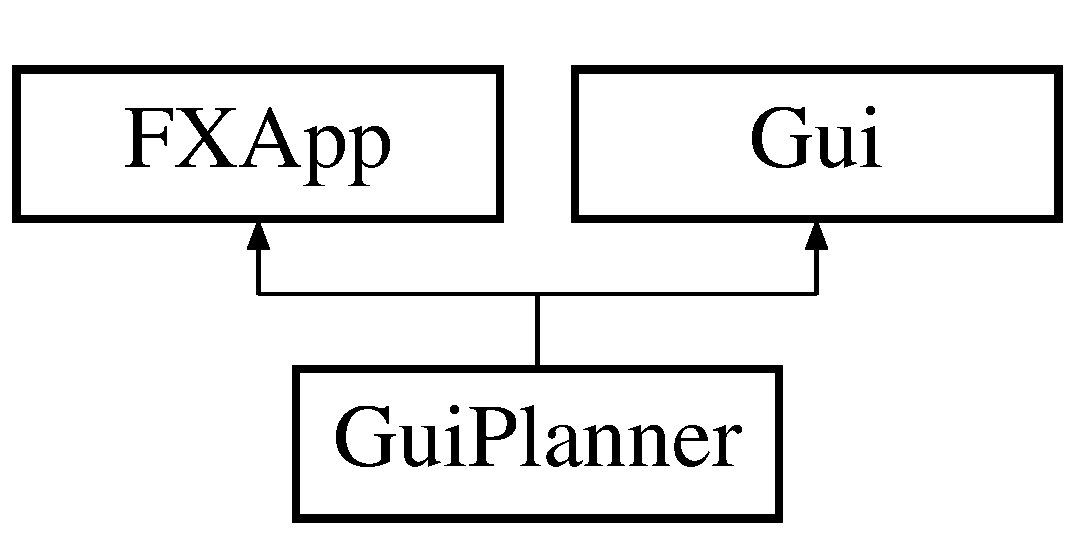
\includegraphics[height=2cm]{classGuiPlanner}
\end{center}
\end{figure}
\subsection*{Public Methods}
\begin{CompactItemize}
\item 
virtual void {\bf Handle\-Events} ()
\begin{CompactList}\small\item\em Process any IO events (may be used by {\bf Render} {\rm (p.\,\pageref{classRender})}).\item\end{CompactList}\item 
virtual void {\bf Button\-Handle} (int b)
\begin{CompactList}\small\item\em Figure out what actions to take based on menu choices.\item\end{CompactList}\item 
{\bf Gui\-Planner} ({\bf Render} $\ast$render, {\bf Planner} $\ast$planner)
\item 
virtual {\bf $\sim$Gui\-Planner} ()
\item 
void {\bf Reset\-Planner} ()
\item 
void {\bf Write\-Graphs} ()
\item 
void {\bf Read\-Graphs} ()
\item 
void {\bf Read\-Animation\-Frames} ()
\item 
void {\bf Write\-Animation\-Frames} ()
\item 
void {\bf Read\-Path} ()
\item 
void {\bf Write\-Path} ()
\item 
void {\bf Draw\-Graphs} ()
\end{CompactItemize}
\subsection*{Public Attributes}
\begin{CompactItemize}
\item 
double {\bf Line\-Width}
\item 
double {\bf PSLine\-Width}
\item 
int {\bf Draw\-Index\-X}
\item 
int {\bf Draw\-Index\-Y}
\item 
{\bf Planner}$\ast$ {\bf Pl}
\end{CompactItemize}
\subsection*{Protected Methods}
\begin{CompactItemize}
\item 
virtual void {\bf Init} ()
\begin{CompactList}\small\item\em Initialize {\bf Gui} {\rm (p.\,\pageref{classGui})} and {\bf Render} {\rm (p.\,\pageref{classRender})}.\item\end{CompactList}\item 
virtual void {\bf Create\-Menu\-Window} ()
\end{CompactItemize}
\subsection*{Protected Attributes}
\begin{CompactItemize}
\item 
{\bf MSLPlanner\-Window}$\ast$ {\bf Window}
\end{CompactItemize}
\subsection*{Friends}
\begin{CompactItemize}
\item 
class {\bf MSLPlot\-Window}
\end{CompactItemize}


\subsection{Constructor \& Destructor Documentation}
\index{GuiPlanner@{Gui\-Planner}!GuiPlanner@{GuiPlanner}}
\index{GuiPlanner@{GuiPlanner}!GuiPlanner@{Gui\-Planner}}
\subsubsection{\setlength{\rightskip}{0pt plus 5cm}Gui\-Planner::Gui\-Planner ({\bf Render} $\ast$ {\em render}, {\bf Planner} $\ast$ {\em planner})}\label{classGuiPlanner_a2}


\index{GuiPlanner@{Gui\-Planner}!~GuiPlanner@{$\sim$GuiPlanner}}
\index{~GuiPlanner@{$\sim$GuiPlanner}!GuiPlanner@{Gui\-Planner}}
\subsubsection{\setlength{\rightskip}{0pt plus 5cm}Gui\-Planner::$\sim$Gui\-Planner ()\hspace{0.3cm}{\tt  [inline, virtual]}}\label{classGuiPlanner_a3}




\subsection{Member Function Documentation}
\index{GuiPlanner@{Gui\-Planner}!ButtonHandle@{ButtonHandle}}
\index{ButtonHandle@{ButtonHandle}!GuiPlanner@{Gui\-Planner}}
\subsubsection{\setlength{\rightskip}{0pt plus 5cm}void Gui\-Planner::Button\-Handle (int {\em b})\hspace{0.3cm}{\tt  [virtual]}}\label{classGuiPlanner_a1}


Figure out what actions to take based on menu choices.



Reimplemented from {\bf Gui} {\rm (p.\,\pageref{classGui_a4})}.\index{GuiPlanner@{Gui\-Planner}!CreateMenuWindow@{CreateMenuWindow}}
\index{CreateMenuWindow@{CreateMenuWindow}!GuiPlanner@{Gui\-Planner}}
\subsubsection{\setlength{\rightskip}{0pt plus 5cm}void Gui\-Planner::Create\-Menu\-Window ()\hspace{0.3cm}{\tt  [protected, virtual]}}\label{classGuiPlanner_b1}


\index{GuiPlanner@{Gui\-Planner}!DrawGraphs@{DrawGraphs}}
\index{DrawGraphs@{DrawGraphs}!GuiPlanner@{Gui\-Planner}}
\subsubsection{\setlength{\rightskip}{0pt plus 5cm}void Gui\-Planner::Draw\-Graphs ()}\label{classGuiPlanner_a11}


\index{GuiPlanner@{Gui\-Planner}!HandleEvents@{HandleEvents}}
\index{HandleEvents@{HandleEvents}!GuiPlanner@{Gui\-Planner}}
\subsubsection{\setlength{\rightskip}{0pt plus 5cm}void Gui\-Planner::Handle\-Events ()\hspace{0.3cm}{\tt  [virtual]}}\label{classGuiPlanner_a0}


Process any IO events (may be used by {\bf Render} {\rm (p.\,\pageref{classRender})}).



Reimplemented from {\bf Gui} {\rm (p.\,\pageref{classGui_a3})}.\index{GuiPlanner@{Gui\-Planner}!Init@{Init}}
\index{Init@{Init}!GuiPlanner@{Gui\-Planner}}
\subsubsection{\setlength{\rightskip}{0pt plus 5cm}void Gui\-Planner::Init ()\hspace{0.3cm}{\tt  [protected, virtual]}}\label{classGuiPlanner_b0}


Initialize {\bf Gui} {\rm (p.\,\pageref{classGui})} and {\bf Render} {\rm (p.\,\pageref{classRender})}.



Reimplemented from {\bf Gui} {\rm (p.\,\pageref{classGui_b1})}.\index{GuiPlanner@{Gui\-Planner}!ReadAnimationFrames@{ReadAnimationFrames}}
\index{ReadAnimationFrames@{ReadAnimationFrames}!GuiPlanner@{Gui\-Planner}}
\subsubsection{\setlength{\rightskip}{0pt plus 5cm}void Gui\-Planner::Read\-Animation\-Frames ()}\label{classGuiPlanner_a7}


\index{GuiPlanner@{Gui\-Planner}!ReadGraphs@{ReadGraphs}}
\index{ReadGraphs@{ReadGraphs}!GuiPlanner@{Gui\-Planner}}
\subsubsection{\setlength{\rightskip}{0pt plus 5cm}void Gui\-Planner::Read\-Graphs ()}\label{classGuiPlanner_a6}


\index{GuiPlanner@{Gui\-Planner}!ReadPath@{ReadPath}}
\index{ReadPath@{ReadPath}!GuiPlanner@{Gui\-Planner}}
\subsubsection{\setlength{\rightskip}{0pt plus 5cm}void Gui\-Planner::Read\-Path ()}\label{classGuiPlanner_a9}


\index{GuiPlanner@{Gui\-Planner}!ResetPlanner@{ResetPlanner}}
\index{ResetPlanner@{ResetPlanner}!GuiPlanner@{Gui\-Planner}}
\subsubsection{\setlength{\rightskip}{0pt plus 5cm}void Gui\-Planner::Reset\-Planner ()}\label{classGuiPlanner_a4}


\index{GuiPlanner@{Gui\-Planner}!WriteAnimationFrames@{WriteAnimationFrames}}
\index{WriteAnimationFrames@{WriteAnimationFrames}!GuiPlanner@{Gui\-Planner}}
\subsubsection{\setlength{\rightskip}{0pt plus 5cm}void Gui\-Planner::Write\-Animation\-Frames ()}\label{classGuiPlanner_a8}


\index{GuiPlanner@{Gui\-Planner}!WriteGraphs@{WriteGraphs}}
\index{WriteGraphs@{WriteGraphs}!GuiPlanner@{Gui\-Planner}}
\subsubsection{\setlength{\rightskip}{0pt plus 5cm}void Gui\-Planner::Write\-Graphs ()}\label{classGuiPlanner_a5}


\index{GuiPlanner@{Gui\-Planner}!WritePath@{WritePath}}
\index{WritePath@{WritePath}!GuiPlanner@{Gui\-Planner}}
\subsubsection{\setlength{\rightskip}{0pt plus 5cm}void Gui\-Planner::Write\-Path ()}\label{classGuiPlanner_a10}




\subsection{Friends And Related Function Documentation}
\index{GuiPlanner@{Gui\-Planner}!MSLPlotWindow@{MSLPlotWindow}}
\index{MSLPlotWindow@{MSLPlotWindow}!GuiPlanner@{Gui\-Planner}}
\subsubsection{\setlength{\rightskip}{0pt plus 5cm}class MSLPlot\-Window\hspace{0.3cm}{\tt  [friend]}}\label{classGuiPlanner_l0}




\subsection{Member Data Documentation}
\index{GuiPlanner@{Gui\-Planner}!DrawIndexX@{DrawIndexX}}
\index{DrawIndexX@{DrawIndexX}!GuiPlanner@{Gui\-Planner}}
\subsubsection{\setlength{\rightskip}{0pt plus 5cm}int Gui\-Planner::Draw\-Index\-X}\label{classGuiPlanner_m2}


\index{GuiPlanner@{Gui\-Planner}!DrawIndexY@{DrawIndexY}}
\index{DrawIndexY@{DrawIndexY}!GuiPlanner@{Gui\-Planner}}
\subsubsection{\setlength{\rightskip}{0pt plus 5cm}int Gui\-Planner::Draw\-Index\-Y}\label{classGuiPlanner_m3}


\index{GuiPlanner@{Gui\-Planner}!LineWidth@{LineWidth}}
\index{LineWidth@{LineWidth}!GuiPlanner@{Gui\-Planner}}
\subsubsection{\setlength{\rightskip}{0pt plus 5cm}double Gui\-Planner::Line\-Width}\label{classGuiPlanner_m0}


\index{GuiPlanner@{Gui\-Planner}!PSLineWidth@{PSLineWidth}}
\index{PSLineWidth@{PSLineWidth}!GuiPlanner@{Gui\-Planner}}
\subsubsection{\setlength{\rightskip}{0pt plus 5cm}double Gui\-Planner::PSLine\-Width}\label{classGuiPlanner_m1}


\index{GuiPlanner@{Gui\-Planner}!Pl@{Pl}}
\index{Pl@{Pl}!GuiPlanner@{Gui\-Planner}}
\subsubsection{\setlength{\rightskip}{0pt plus 5cm}{\bf Planner} $\ast$ Gui\-Planner::Pl}\label{classGuiPlanner_m4}


\index{GuiPlanner@{Gui\-Planner}!Window@{Window}}
\index{Window@{Window}!GuiPlanner@{Gui\-Planner}}
\subsubsection{\setlength{\rightskip}{0pt plus 5cm}{\bf MSLPlanner\-Window} $\ast$ Gui\-Planner::Window\hspace{0.3cm}{\tt  [protected]}}\label{classGuiPlanner_n0}




The documentation for this class was generated from the following files:\begin{CompactItemize}
\item 
{\bf guiplanner.h}\item 
{\bf guiplanner.C}\end{CompactItemize}
